\section{Diagramma delle classi}
\label{ch:diagrammaClassi}

\subsection{Definizione delle classi}

 Le figure seguenti riportano i nomi reali dei campi Mongoose implementati. Nelle risposte JSON l'identificativo \`e esposto come \texttt{\_id} (con \texttt{self} come link canonico). 
    Ogni classe riporta oltre agli attributi anche i metodi (operazioni). La mappatura completa metodo $\rightarrow$ endpoint REST \`e nel capitolo~\ref{ch:dalClassDiagramAlleAPI}.

    \subsection*{1. Utente (\texttt{User})}
        La classe \texttt{Utente} rappresenta qualsiasi utente del sistema. Il ruolo viene memorizzato nell'attributo \texttt{role} (enum \texttt{admin} o \texttt{operator}): l'operatore tecnico gestisce edifici, sensori e allarmi mentre l'amministratore possiede il controllo totale (gestione utenti, inviti, esportazione dati, configurazione di sistema oltre ai privielgi dell'operatore tecnico).
        \begin{figure}[H]
            \centering
            \includegraphics[width=0.5\textwidth]{../images/ClassDiagram/ClassiWattguard-Utente.png}
            \caption{Classe \texttt{Utente}: attributi e metodi}
        \end{figure}

    \subsection*{2. Invito (\texttt{Invite})}
        La classe \texttt{Invito} rappresenta l'invito inviato via email a un nuovo utente, con il relativo token e la scadenza (7 giorni). Permette all'amministratore di creare gli account senza condividerne le credenziali.
        \begin{figure}[H]
            \centering
            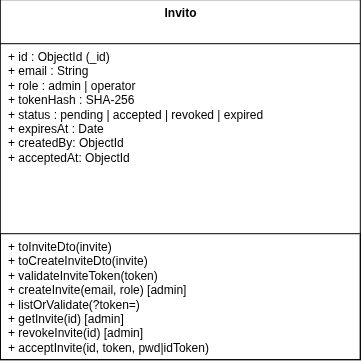
\includegraphics[width=0.5\textwidth]{../images/ClassDiagram/ClassiWattguard-Invito.png}
            \caption{Classe \texttt{Invito}: attributi e metodi}
        \end{figure}

    \subsection*{3. TokenResetPassword (\texttt{PasswordResetToken})}
        La classe \texttt{TokenResetPassword} rappresenta il token monouso generato per la procedura di reset della password. Il token scade dopo 1 ora (durata impostata dal service).
        \begin{figure}[H]
            \centering
            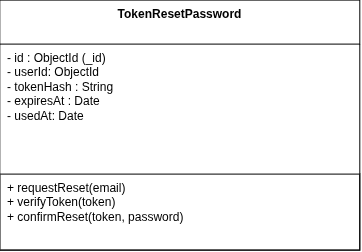
\includegraphics[width=0.5\textwidth]{../images/ClassDiagram/ClassiWattguard-TokenResetPassword.png}
            \caption{Classe \texttt{TokenResetPassword}: attributi e metodi}
        \end{figure}

    \subsection*{4. Edificio (\texttt{Building})}
        La classe \texttt{Edificio} rappresenta la struttura pubblica monitorata dal sistema. Oltre ai dati anagrafici e strutturali, memorizza la posizione geografica come punto \texttt{GeoJSON} (longitudine/latitudine) e conserva il riferimento alla propria tipologia.
        \begin{figure}[H]
            \centering
            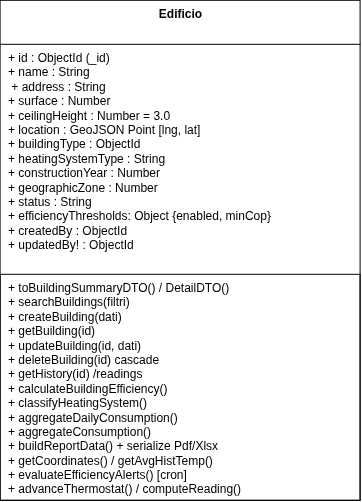
\includegraphics[width=0.5\textwidth]{../images/ClassDiagram/ClassiWattguard-Edificio.png}
            \caption{Classe \texttt{Edificio}: attributi e metodi}
        \end{figure}

    \subsection*{5. TipologiaEdificio (\texttt{BuildingType})}
        La classe \texttt{TipologiaEdificio} rappresenta le categorie di edifici (ad esempio ``scuola'', ``ufficio'', ``palestra''). Il nome è univoco; una tipologia può essere eliminata solo se non è più utilizzata da alcun edificio.
        \begin{figure}[H]
            \centering
            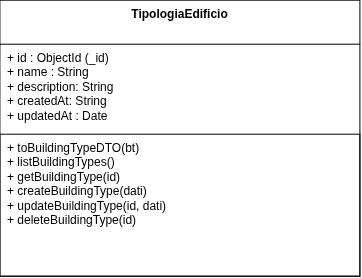
\includegraphics[width=0.5\textwidth]{../images/ClassDiagram/ClassiWattguard-TipologiaEdificio.png}
            \caption{Classe \texttt{TipologiaEdificio}: attributi e metodi}
        \end{figure}

    \subsection*{6. Sensore (\texttt{Sensor})}
        La classe \texttt{Sensore} rappresenta un dispositivo IoT installato in un edificio. Il riferimento all'edificio \`e memorizzato nel campo \texttt{building} (nome reale nel codice). La tipologia è un attributo enumerato (temperatura interna, temperatura esterna, contatore elettrico, contatore gas); le soglie di allarme \texttt{minThreshold} e \texttt{maxThreshold} sono attributi del sensore stesso. L'ultima rilevazione è memorizzata in forma denormalizzata nell'attributo \texttt{lastReading} per garantire letture immediate, mentre lo storico completo è nella classe \texttt{Rilevazione}.
        \begin{figure}[H]
            \centering
            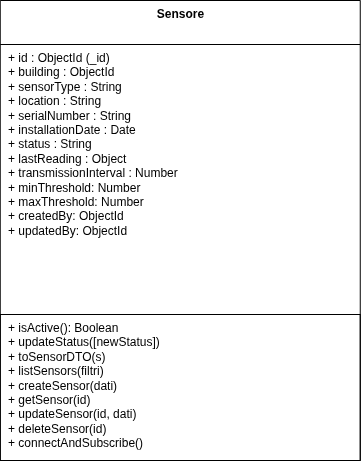
\includegraphics[width=0.5\textwidth]{../images/ClassDiagram/ClassiWattguard-Sensore.png}
            \caption{Classe \texttt{Sensore}: attributi e metodi}
        \end{figure}


    \subsection*{7. Rilevazione (\texttt{SensorReading})}
        La classe \texttt{Rilevazione} rappresenta una singola misurazione effettuata da un sensore in un determinato istante. È una collezione che mantiene lo storico dei dati necessario alle analisi di andamento, efficienza e all'esportazione. Un TTL di 365 giorni rimuove automaticamente le rilevazioni pi\`u vecchie.
        \begin{figure}[H]
            \centering
            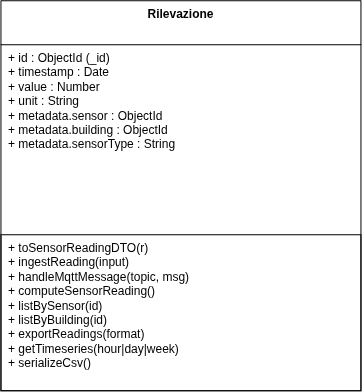
\includegraphics[width=0.5\textwidth]{../images/ClassDiagram/ClassiWattguard-Rilevazione.png}
            \caption{Classe \texttt{Rilevazione}: attributi e metodi}
        \end{figure}

    \subsection*{8. Allarme (\texttt{Alert})}
        La classe \texttt{Allarme} rappresenta una notifica generata automaticamente dal sistema quando una rilevazione supera le soglie configurate sul sensore oppure quando viene rilevata un'anomalia di efficienza (COP sotto soglia). 
        \begin{figure}[H]
            \centering
            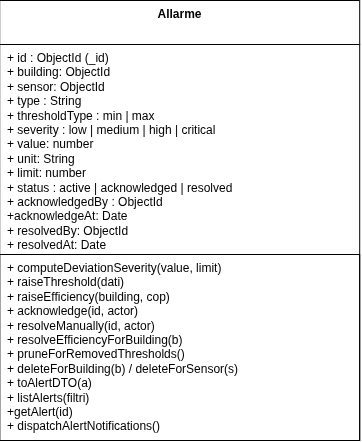
\includegraphics[width=0.5\textwidth]{../images/ClassDiagram/ClassiWattguard-Allarme.png}
            \caption{Classe \texttt{Allarme}: attributi e metodi}
        \end{figure}

    \subsection*{9. Configurazione Sistema (\texttt{SystemConfig})}
        La classe \texttt{ConfigurazioneSistema} è un documento \emph{singleton} solo per convenzione applicativa che conserva la configurazione globale del sistema (intervallo di polling del frontend, abilitazione delle notifiche email, giorni di conservazione dei dati storici).
        \begin{figure}[H]
            \centering
            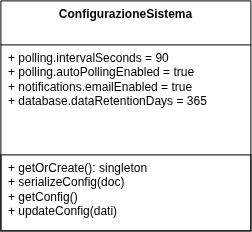
\includegraphics[width=0.5\textwidth]{../images/ClassDiagram/ClassiWattguard-ConfigurazioneSistema.png}
            \caption{Classe \texttt{ConfigurazioneSistema}: attributi e metodi}
        \end{figure}

\newpage

\subsection{Diagramma delle classi complessivo}
    Di seguito il diagramma delle classi complessivo con tutte le classi presentate e le relative relazioni (da rigenerare in base alle definizioni corrette).
    \begin{figure}[H]
        \centering
        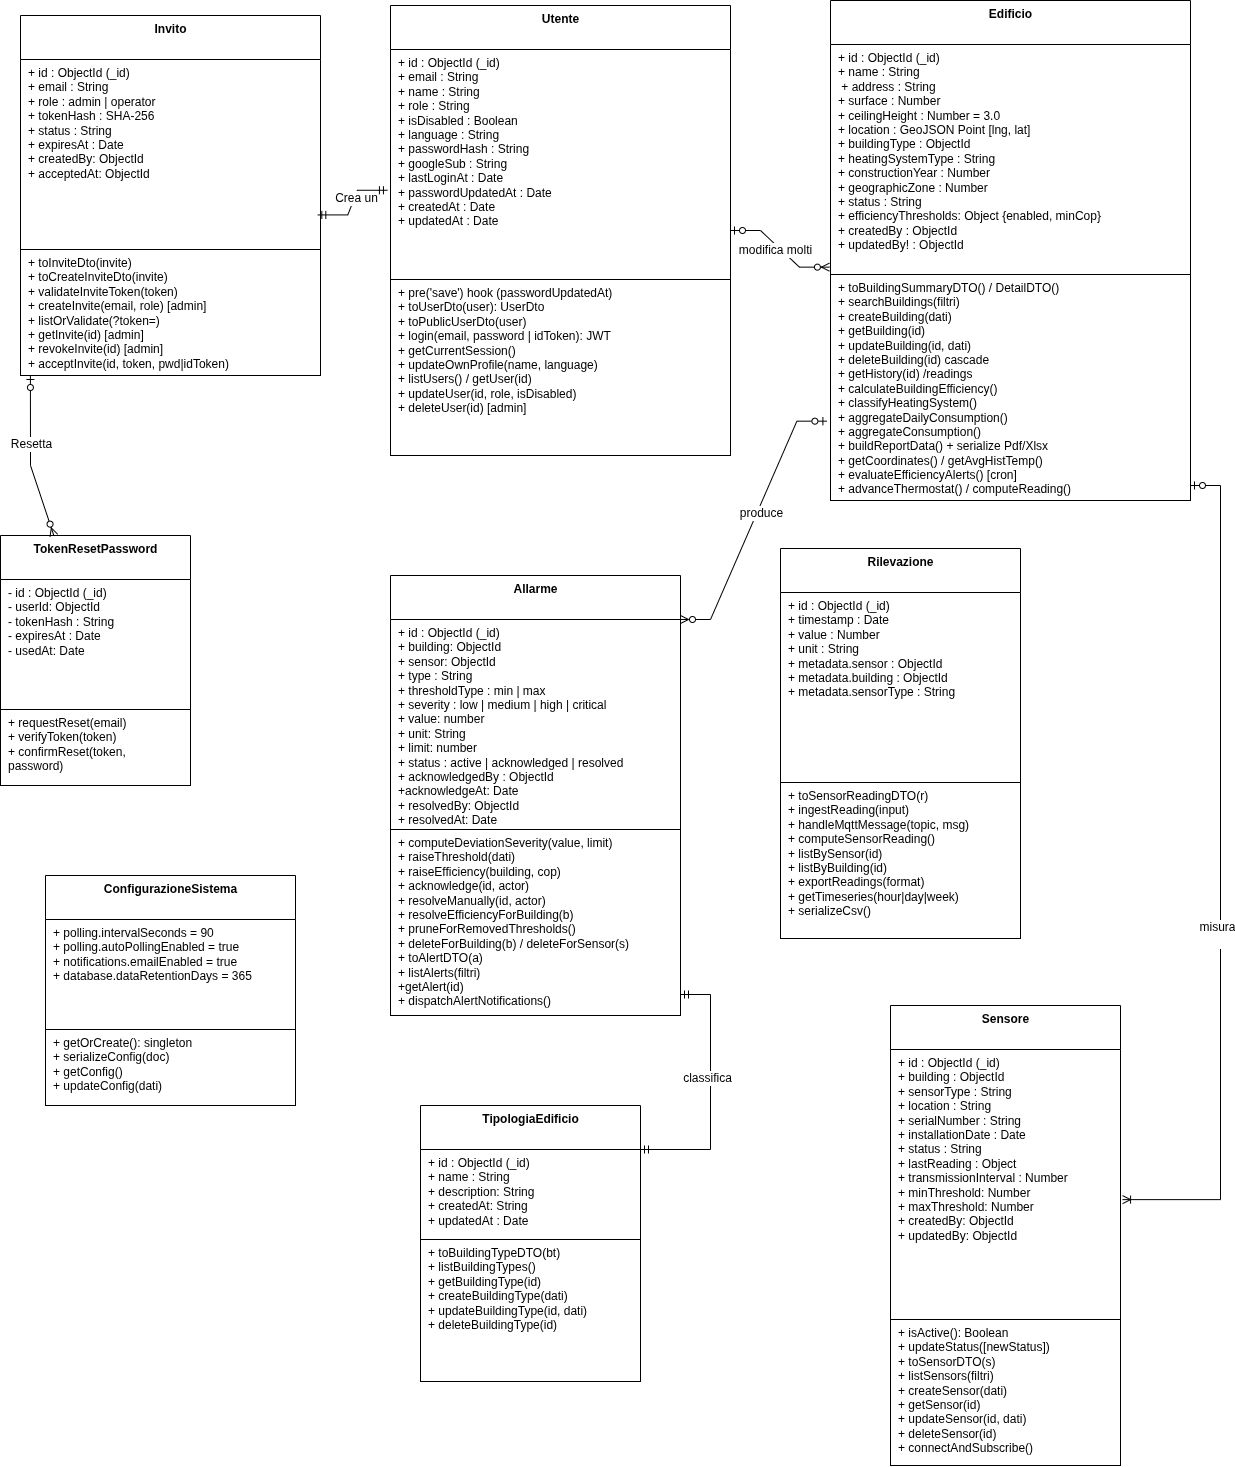
\includegraphics[width=1\textwidth]{../images/ClassDiagram/ClassiWattguard-DiagrammaGenerale.png}
        \caption{Diagramma delle classi complessivo di \texttt{WattGuard}}
    \end{figure}
